\subsection{Hechos y teoremas \'utiles}
\begin{multicols}{2}
\begin{center}
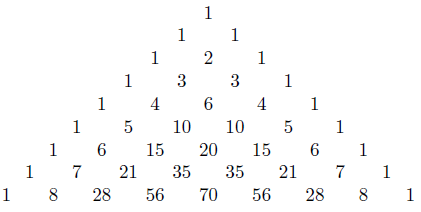
\includegraphics[width=65mm]{./combinatory/pascal}
\end{center}
\textbf{Permutaciones:}

El n\'umero de permutaciones (posibles reordenamientos) de $n$ objetos es $n!$\\
\textbf{Subconjuntos:}

El n\'umero de subconjuntos de $k$ elementos formados a partir de uno de $n$ elementos es ${n \choose k} = \frac{n!}{(n-k)!k!}$.\\
\textbf{Subconjuntos ordenados:}

El n\'umero de subconjuntos ordenados de $k$ elementos formados a partir de uno de $n$ elementos es $n(n-1)\cdots (n-k+1)=\frac{n!}{(n-k)!}$.\\
\textbf{El teorema binomial:}

Los coeficientes de $x^{n-k}y^k$ en la expansi\'on de $(x+y)^n$ es el coeficiente binomial ${n \choose k} = \frac{n!}{(n-k)!k!}$. En otras palabras tenemos la identidad: \[ (x+y)^n =  {n \choose 0}x^n+{n \choose 1}x^{n-1}y+\cdots +{n \choose n-1}xy^{n-1}+{n \choose n}y^n \]

\textbf{Algunas propiedades de los coeficientes binomiales:}
\begin{itemize}
\item Simetr\'ia

\[{n \choose k} = {n \choose n-k}\]

\item Identidad de Pascal

\[{n-1 \choose k-1} + {n-1 \choose k} = {n \choose k}\]

\item Subconjuntos de un conjunto

\[\sum\limits_{k=0}^n{n \choose k} =  2^n\]

\item Identidad de Vandermonde

\[{m+n \choose r} = \sum\limits^r_{k=0}{m \choose r-k}{n \choose k}\]
\end{itemize}
\end{multicols}
\subsection{Como generar el n\'umero de combinaciones}
Consigue $n$ combinado $k$ en $O(n^2)$ por programaci\'on din\'amica:
\codigofuente{./combinatory/ManejadorCombinaciones.java}